\documentclass{beamer}

\usepackage[british]{babel}
\usepackage{graphicx,hyperref,ru,url}
\usepackage{amsmath}
\usepackage{amssymb}
\usepackage{biblatex}
\newcommand{\R}{\mathbb{R}}
\usepackage{adjustbox} % Shrink stuff

\usepackage{algorithmicx}
\usepackage{algpseudocode}
\usepackage{algorithm}

\usepackage{pythonhighlight}

\graphicspath{
	{images/}
} 
\bibliography{main.bib}
% Fancy fit image command with optional caption
\makeatletter
\newcommand{\fitimage}[2][\@nil]{
	\begin{figure}
		\begin{adjustbox}{width=0.5\textwidth, totalheight=\textheight-1\baselineskip-3\baselineskip,keepaspectratio}
			\includegraphics{#2}
		\end{adjustbox}
		\def\tmp{#1}%
		\ifx\tmp\@nnil
		\else
		\caption{#1}
		\fi
	\end{figure}
}
 

% RU style for Beamer
% The title of the presentation:
%  - first a short version which is visible at the bottom of each slide;
%  - second the full title shown on the title slide;
\title[On Solving PDEs with NN]{
  Solving Partial Differential Equations with
  Uncertainties Using Neural-Networks\\(A surrogate forward model)}

% Optional: a subtitle to be dispalyed on the title slide
%\subtitle{Institute for Advanced Studies in Basic Sciences}

% The author(s) of the presentation:
%  - again first a short version to be displayed at the bottom;
%  - next the full list of authors, which may include contact information;
\author[Sajed N. Zarrinpour]{
  Sajed N. Zarrinpour \\\medskip
  {\small Dr Khadijeh Nedaiasl, Dr Parvin Razaghi} \\ 
  {\small \url{sa.zarrinpour@iasbs.ac.ir}}}

% The institute:
%  - to start the name of the university as displayed on the top of each slide
%    this can be adjusted such that you can also create a Dutch version
%  - next the institute information as displayed on the title slide
\institute[IASBS]{
  Institute for Advanced Studies in Basic Sciences}

% Add a date and possibly the name of the event to the slides
%  - again first a short version to be shown at the bottom of each slide
%  - second the full date and event name for the title slide
\date[\today]{
  May 2020 }

\begin{document}

\begin{frame}
  \titlepage
\end{frame}

\begin{frame}
  \frametitle{Outline}

  \tableofcontents
\end{frame}

% Section titles are shown in at the top of the slides with the current section 
% highlighted. Note that the number of sections determines the size of the top 
% bar, and hence the university name and logo. If you do not add any sections 
% they will not be visible.
\section{Introduction}


\begin{frame}
	\frametitle{}

	\textbf{``The key is in not spending time, but in investing it''}\centering\\
	\em - Stephen R. Covey. 
	
\end{frame}
\begin{frame}
	\frametitle{}
	\textbf{Use Case Example}\centering\\
	\textit{Breast Cancer}\centering\\
\end{frame}
\begin{frame}
	\frametitle{Use Case: Breast Cancer}
	
	\begin{block}{MRI-guided biopsy}
		\fitimage[{\tiny https://healthmanagement.org/products/view/breast-biopsy-mri-coil-sentinelle-hologic}]{images/MRI-guided-byopsi.jpg}
	\end{block}		
\end{frame}

\begin{frame}
	\frametitle{Use Case: Breast Cancer}
	
	\begin{block}{MRI-guided biopsy sample image}
		\fitimage[{\tiny https://www.cedars-sinai.edu/Patients/Programs-and-Services/Imaging-Center/For-Patients/Exams-by-Procedure/MRI/MR-Guided-Breast-Biopsy/}]{images/Breast-mr-2.jpg}
	\end{block}		
\end{frame}

\begin{frame}
	\frametitle{Use Case: Breast Cancer}
	
	\begin{block}{Ultra sound imaging}
		\fitimage[{\tiny https://www.philips.com/a-w/about/news/archive/standard/news/press/2018/20181025-philips-debuts-integrated-breast-ultrasound-solution-to-make-exams-easier-and-faster-for-patients-and-clinicians.html}]{images/UltraSounfImaging.jpg}
	\end{block}		
\end{frame}

\begin{frame}
	\frametitle{Use Case: Breast Cancer}
	
	\begin{block}{Ultra sound sample image}
		\fitimage[{\tiny https://www.radiology.pitt.edu/node/225}]{images/ultra-sound-image-sample.png}
	\end{block}		
\end{frame}

\begin{frame}
	\frametitle{Use Case: Breast Cancer}
	
	\begin{block}{FEM Model $\sim$ 2 hours}
		\fitimage[{\tiny https://aapm.onlinelibrary.wiley.com/doi/10.1002/mp.12673}]{images/FEM-Model-of-Breast.png}
	\end{block}		
\end{frame}

\begin{frame}
	\frametitle{Use Case: Breast Cancer}
	
	\begin{block}{FEM - ML Model $\sim$ 0.2 seconds}
		\fitimage[{\tiny https://www.sciencedirect.com/science/article/abs/pii/S0010482517303177}]{images/FEM-ML-model.jpg}
	\end{block}		
\end{frame} 

\begin{frame}
	\frametitle{}
	\textbf{What are the bottlenecks?}\centering\\
\end{frame}

\section{Background Information}
\begin{frame}
  \frametitle{Finite Element Method}

  \begin{block}{Poisson Equation on Unit Square - Strong Form}
  	\begin{align*} 	
  	\begin{array}{rcr}
	  	-\Delta u = &f(x)&\text{ ,in }\Omega = [0\times 1] \times [0\times 1] - [0, 1) \\ 
	  	u = &0 &\text{ ,on }\partial \Omega 
  	\end{array}
  	\end{align*}	
  \end{block}
\end{frame}


\begin{frame}
	\frametitle{Finite Element Method}	
	\begin{block}{Poisson Equation on Unit Square - Weak Form}		
		$\sum_{i=1}^{M} c_i <\phi_i,\phi_j> = <f,\phi_j> \hspace{30pt} i=1,...,M$,	
				
		where	
		
		 $u_h = \sum_{i=1}^{M} c_i \phi_i \hspace{5pt} and \in V_h=span\{\phi_i\}_{i=1}^{M}$		
	\end{block}	
\end{frame}

\begin{frame}
	\frametitle{}
	
	\textbf{Removing the bottleneck.}\centering\\
	\textit{Is It Possible?}\centering\\
	
\end{frame}


\begin{frame}
	\frametitle{Possibility}
	
	\begin{block}{Universal Approximation Theorem}
		Let $\phi:\R \to \R$ be a non-constant, bounded, and continuous function. Let $I_m$ denote the m-dimensional unit hypercube $[0, 1]^m$. The space of real-valued continuous functions on $I_m$ is denoted by $C(I_m)$. Then, given any $\epsilon >0$ and any function $f \in C(I_m)$, there exist an integer N, real constants $v_i, b_i \in \R$ and real vectors $w_i \in \R^m$ for i=1,...,N, such that we may have define :
		
		$F(x) = \sum_{i=1}^{N} v_i \phi(w_{i}^{T}x + b_i)$
		as an approximate realization of the function f; that is,
		$|F(x)-f(x)| < \epsilon$
		for all $x\in I_m$. 
	\end{block}	
\end{frame}

\begin{frame}
	\frametitle{Possibility}
	
	\begin{block}{Universal Approximation Theorem}	
		For any Lebesgue-integrable function $f:\R^{n}\rightarrow \R$ and any $\epsilon > 0$ , there exists a fully-connected ReLU network $\mathcal{A}$ with width $d_{m}\leq {n+4}$, such that the function $F_{\mathcal{A}}$ represented by this network satisfies:\\
		 $\int_{\R}^{} \|f(x) - F_{A}(A)\| dx < \epsilon $
	\end{block}	
\end{frame}

\begin{frame}
	\frametitle{}
	
	\textbf{Alright. Where to begin?!}\centering\\
	
\end{frame}

\begin{frame}
	\frametitle{Neural-Network}	
	  \begin{block}{Artificial Neuron}
		\begin{itemize}
			\item <1- > \textbf{W}eight, \textbf{b}ias 
			\item <2- > Activation function (\textbf{$\psi$})
		\end{itemize}	
	\end{block}
\end{frame}

\begin{frame}
	\frametitle{Neural-Network}
		  \begin{block}{Artificial Neuron}
			\textbf{$\psi(WX+b)$}\centering\\	
	   	\end{block}	
\end{frame}


\begin{frame}
	\frametitle{}
	
	\textbf{Different Combinations $\sim$ Different Networks}\centering\\
	\textit{Let's see it in action!}\centering\\
	
\end{frame}

\begin{frame}
	\frametitle{Deep Ritz Method}
	
	\begin{block}{Poisson Equation - Neural Networks Form}
	$u_{\theta}(x) = a . f_{n}(x) \circ ... \circ f_{1}(x) +b$ \\
	where \\
	$f_{i}(x) = \phi(W_i2 . \phi(W_i1 . x + b_{i1}) + b_{i2}) + x $ and $a \in \R^m, b\in\R $ \\
	and $\phi(x) = \max\{x^3,0\}$
	\end{block}	
\end{frame}

\begin{frame}
	\frametitle{Deep Ritz Method}
	\begin{figure}
		\begin{block}{(a) DRM - 811 parameter, (b) FDM - 1681 parameter}		
		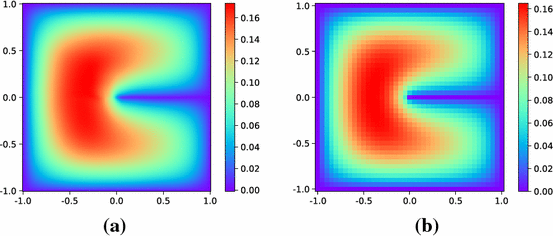
\includegraphics[width=\textwidth,height=\textheight,keepaspectratio]{DRMvsFDM.png}
		\caption{https://arxiv.org/abs/1710.00211}
	\end{block}
	\end{figure}
\end{frame}

\begin{frame}
	\frametitle{Neural-Network}
	\begin{block}{How It Works}
		\begin{itemize}
			\item<1- > structure
			\item<2- > loss function
		\end{itemize}
	\end{block}
\end{frame}

\begin{frame}
	\frametitle{}
	
	\textbf{Are You READY?!}\centering\\
	\textit{Let's dive deep!}\centering\\
	
\end{frame}
\section{Problem Definition \& Results}
\begin{frame}
	\frametitle{}
	
	\textbf{Linear Case}\centering\\
	\textit{effective conductance in inhomogeneous media}\centering\\
	
\end{frame}

\begin{frame}
	\frametitle{Linear Case}
	
	\begin{block}{Effective Conductance}
		\begin{align*} 	
		\begin{array}{rll}
		A_{\mathrm{eff}}(a) = &\min_{u(x)} \int_{[0,1]^d} a(x) ||\nabla u(x) + \xi||_{2}^{2} \mathrm{d}x.&\text{ ,in }\Omega = [0\times 1]\\ 
		u(0) = &u(n) &\text{ ,on }\partial \Omega 
		\end{array}
		\end{align*}	
	\end{block}
	\begin{block}{Final result}
	$mean(A_{\mathrm{eff}}(a)) = 0.76800650$,\\
	With $1.021 \times 10^{-3}$ $L^2$-Error
	\end{block}
\end{frame}

\begin{frame}
	\frametitle{}	
	\begin{block}{Steps}
		\begin{itemize}
			\item Data Set Generation 
		\end{itemize}	
	\end{block}
\end{frame}

\begin{frame}
	\frametitle{Linear Case}
	
	\begin{block}{Minimization Form}
		\begin{align*} 	
		\begin{array}{rll}
		A_{\mathrm{eff}}(a) = &\min_{u(x)} \int_{[0,1]^d} a(x) ||\nabla u(x) + \xi||_{2}^{2} \mathrm{d}x.&\text{ ,in }\Omega = [0\times 1]\\ 
		u(0) = &u(n) &\text{ ,on }\partial \Omega 
		\end{array}
		\end{align*}	
	\end{block}
	\begin{block}{Equivalent PDE Form}	
		\begin{align*}
	-\nabla \cdot (a(x)(\nabla u(x)+\xi)) = &0
		\end{align*}	
	\end{block}
\end{frame}

\begin{frame}
	\frametitle{Linear Case}
	
	\begin{block}{Calculate $u_a$}	
		\begin{align*}
		(L_a u)_i &:= \sum_{k=1}^{d} \frac{-a_{i+\frac{1}{2}e_k} u_{i+e_k} + (a_{i-\frac{1}{2}e_k} + a_{i+\frac{1}{2}e_k})u_i - a_{i-\frac{1}{2}e_k} u_{i-e_k} }{h^2}\\
		(b_a)_i &:= \sum_{k=1}^{d} \frac{\xi_k (a_{i+\frac{1}{2}e_k} - a_{i-\frac{1}{2}e_k})}{h} 
		\end{align*}	
	\end{block}
	\begin{block}{Effective Conductance}	
	\begin{align*}
		A_{\mathrm{eff}}(a) = &h^d (u_a^T L
u_a - 2u^T_a b_a + a^T 1)
	\end{align*}	
\end{block}
\end{frame}

\begin{frame}
	\frametitle{}	
	\begin{block}{Steps}
		\begin{itemize}
			\item  Data Set Generation 
			\item  Neural-Network Model
		\end{itemize}	
	\end{block}
\end{frame}

\begin{frame}
	\frametitle{Linear Case}
		\begin{figure}[h!]
			{
				\centering
				\def\svgwidth{\columnwidth}
				\scalebox{1}{\input{images/ECIM_NN_Structure.pdf_tex}}
				\caption{Neural-Network architecture}
			}
		\end{figure}	
\end{frame} 


\begin{frame}
	\frametitle{Linear Case}
	\begin{figure}[h!]
		{
			\centering
			\def\svgwidth{\columnwidth}
			\scalebox{.5}{\input{images/ECIM_bar.pdf_tex}}
			\caption{committed error per sample over the prediction set}
		}
	\end{figure}	
\end{frame} 
\begin{frame}
	\frametitle{Linear Case}
	\begin{figure}[h!]
		{
			\centering
			\def\svgwidth{\columnwidth}
			\scalebox{.5}{\input{images/ECIM_percentages.pdf_tex}}
			\caption{committed error per sample over the prediction set distribution}
		}
	\end{figure}	
\end{frame} 

\begin{frame}
	\frametitle{}
	
	\textbf{Nonlinear Case}\centering\\
	\textit{Nonlinear Shr\"{o}dinger equation with inhomogeneous background potential}\centering\\
	
\end{frame}
\begin{frame}
	\frametitle{Nonlinear Case}
	
	\begin{block}{Shr\"{o}dinger Equation}
		\begin{align*} 	
		\begin{array}{rll}
		-\Delta u(x) + a(x)u(x) + \sigma u(x)^3 = &E_0 u(x) &\text{ ,in }\Omega = [0\times 1]^2\\ 
		\int_{[0,1]^2}u(x)^2 \mathrm{d}x = &1\\
		u(0) = &u(n) &\text{ ,on }\partial \Omega 
		\end{array}
		\end{align*}	
	\end{block}
		\begin{block}{Final result}
		$mean(E) = 10.17474556$,\\
		With $7.235 \times 10^{-5}$ $L^2$-Error
	\end{block}
\end{frame}

\begin{frame}
	\frametitle{}	
	\begin{block}{Steps}
		\begin{itemize}
			\item Data Set Generation 
		\end{itemize}	
	\end{block}
\end{frame}


\begin{frame}
	\frametitle{Nonlinear Case}
	
	\begin{block}{FDM}	
		\begin{align*}
		&(Lu)_i + a_i u_i + \sigma u_{i}^3 = E_0 u_i, \\
		&\sum_{i=1}^{n^2} u_{i}^2 h^2 = 1,\\
		&(lu)_i := \sum_{k=1}^{d} \frac{-u_{i+e_{k}} + 2u_i - u_{i-e_{k}}}{h^2}
		\end{align*}	
	\end{block}
\end{frame}

\begin{frame}
	\frametitle{}	
	\begin{block}{Steps}
		\begin{itemize}
			\item  Data Set Generation 
			\item  Neural-Network Model
		\end{itemize}	
	\end{block}
\end{frame}

\begin{frame}
	\frametitle{Nonlinear Case}
	
	\begin{figure}[h!]
		{
			\centering
			\def\svgwidth{\columnwidth}
			\scalebox{1}{\input{images/NLSE_NN_Structure.pdf_tex}}
			\caption{Single convolutional layer.}
		}
	\end{figure}	
\end{frame}

\begin{frame}
	\frametitle{Nonlinear Case}
	\begin{block}{Periodic Padding Psudo Code}
		\inputpython{./periodicpadding.py}{1}{14}
	\end{block}
\end{frame}


\begin{frame}
	\frametitle{Nonlinear Case}
	\begin{figure}[h!]
		{
			\centering
			\def\svgwidth{\columnwidth}
			\scalebox{.5}{\input{images/bar.pdf_tex}}
			\caption{committed error per sample over the prediction set}
		}
	\end{figure}	
\end{frame} 
\begin{frame}
	\frametitle{Nonlinear Case}
	\begin{figure}[h!]
		{
			\centering
			\def\svgwidth{\columnwidth}
			\scalebox{.5}{\input{images/percentages.pdf_tex}}
			\caption{committed error per sample over the prediction set}
		}
	\end{figure}	
\end{frame} 



\section{Conclusion}
\begin{frame}
	\frametitle{Conclusion}
	\begin{itemize}
		\item <1- > Bypassing the calculation of the basis
		\item <2- > Better accuracy in less cost
		\item <3- > Almost the same for Linear and Nonlinear
	\end{itemize}
\end{frame}

\begin{frame}
	\frametitle{Future Works}
	\begin{itemize}
		\item <1- > Studying methods for label scaling/normalization
		\item <2- > Incorporating more physical knowledge to the model
		\item <3- > Using this method for simulation of soft tissue deformation
	\end{itemize}
\end{frame}

\begin{frame}
  \frametitle{Q\&A}
\textbf{"Ask, and it shall be given you!"}\centering\\
\em Matthew 7:7
\end{frame}
\section{References}
\begin{frame}
	\frametitle{References}
	\begin{itemize}
		\item \href{https://www.semanticscholar.org/paper/Solving-PDE-problems-with-uncertainty-using-Khoo-Lu/ffacc17153bf122cc8a726adca6b468cd5fecb54}{Solving PDE problems with uncertainty using neural-networks}
		\item \href{https://arxiv.org/pdf/1710.00211.pdf}{The Deep Ritz Method}
		\item \href{https://www.sciencedirect.com/science/article/abs/pii/S0010482517303177}{A finite element-based machine learning approach for modeling the mechanical behavior of the breast tissues under compression in real-time}
		\item \href{https://en.wikipedia.org/wiki/Universal_approximation_theorem}{Universal Approximation Theorem}
		\item \href{https://www.actitime.com/time-management/best-time-quotes/}{Quotes about the time}	
\end{itemize}
\end{frame}

\end{document}
